\chapter{The Insieme Compiler} \label{cap:compiler}
\index{Compiler}

\section{Overview}

To be noted:
\begin{itemize}
  \item The compiler is a library, not a framework or a single executable with a
  tone of flags
  \item Overview on the various modules
\end{itemize}

\subsection{Architecture}
\subsection{Coding Standards}
\subsection{Source Code Organization}
\subsection{Building a Simple Optimizing Compiler}
\label{cap:compiler:sec:overview:sub:building} TODO: add an example loading
code, changing something stupid and generating output code.

\section{The Utilities}
\subsection{Logging}
\subsection{Compiler}
\subsection{Lua}
\subsection{Others}
\subsubsection{Container Utilities}
\subsubsection{Set Utilities}
\subsubsection{Cache Utilities}
\subsubsection{String Utilities}
\subsubsection{Type Traits}

\section{The Core}
The main obligation of the core module is to provide the data structures
required to represent program code based on the Insieme Parallel Intermediate
Representation (INSPIRE). In addition to the raw data structures, a set of
primitives and utilities to inspect, address, analyse, manipulate and load/store
IR codes are offered to enable a high level interaction with the sometimes rather
low-level elements. Throughout the remaining compiler modules, this
representation is used as an exchange format when dealing with programs.

\subsection{The Core's Contributions}
\subsubsection{Representation}
The compilers intermediate representation is a formal, Turing-complete,
high level programming language specified within the Insieme IR
Language Specification \cite{insieme_ir_spec}. Internally, the various
constructs required to represent programs are modeled using nodes within a DAG 
(see \ref{sec:Compiler.Core.NodesAndManagers}). Each node has a certain type
(e.g. a variable, a for-loop or an array-type) and a list of child-nodes
representing parameters of the individual node types (e.g. value type, loop
body or length or an array). Although virtually representing a tree, the nodes
are physically organized withing a DAG since many sub-trees within a program
representation (e.g. reused struct types or functions) are identical. By using a
DAG structure, these unnecessary redundancy can be avoided by sharing common
sub-trees. However, as a consequence of the sharing, all nodes within the DAG
have to be immutable.

\subsubsection{Construction}
Every data structure needs to be constructed at some point. All nodes of an IR
DAG can be constructed using static factories associated to the corresponding
node types (see \ref{sec:Compiler.Core.NodesAndManagers.Factories}). In many
cases, this is a very cumbersome way of constructing IR codes since various
frequently used constructs involve the construction of several nodes.
Furthermore, proper typing of expressions is required. Therefore, a builder has
been implemented supporting the construction of typical, frequently used IR
fragments. Its internal organization is covered within section
\ref{sec:Compiler.Core.Builder}. However, for more extensive code sections like
a simple loop nest, using the builder still requires a considerable amount of
coding effort making the resulting code unreadable. Also, it is sometimes next
to impossible to deduce from the code what has been constructed. Therefore, an
\textit{IR Parser} converting a string-based input IR code is provided to offer
a convenient mean to build larger IR constructs. For details see
\ref{sec:Compiler.Core.Parser}.

\subsubsection{Addressing}
Nodes within the IR of a program can be addressed using two distinct means. The
simple one is by obtaining a pointer to the corresponding node. However, in some
cases this is not sufficient, since a pointer to a node within a DAG does not
allow to distinguish multiple usages of the same, shared structure. For
instance, a pointer to a variable node is simply referencing this variable.
Since the same node is commonly referenced by any location the variable is
touched by, a pointer does not allow to determine which actual ``position'' in a
program is to be addressed. However, pointers are a cheap way of addressing
elements and in many cases the actual context is not important. If, however, the
context gets important, \textit{NodeAddresses} can be used. Unlike pointers,
addresses model the full path from some root node (not necessarily the global
root node) to an addressed node within the virtual IR tree. Therefore, all the
context information is available. Addresses may for instance be used when aiming
for replacing specific sections of a program -- sections which might be present
in an identical form within the program at different places. More regarding the
implementation of addressing means in the IR is covered within the corresponding
section \ref{sec:Compiler.Core.PointersAndAddresses}. Section
\ref{sec:Compiler.Core.Visitors} lists the various means offered to iterate over
(sub-sections) of an IR tree using \textit{Visitors} while section
\ref{sec:Compiler.Core.Mappers} covers the basic mechanism for ``mutating'' IR
constructs based on Node \textit{Mappers}.

\subsubsection{Extensions}
Not every construct defined by the INSPIRE language is converted into a
specialized IR node. For instance, basic types (integers,
floats, specialized arrays, \ldots) and a list of operations manipulating
values of those types (addition, array accesses, \ldots) are integrated using a
standardised procedure. The implementation of the procedure used for defining
the core language (also known as Lang-Basic) and various, special-purpose
language extensions are covered within section
\ref{sec:Compiler.Core.LangBasic}.

\subsubsection{IO}
Section \ref{sec:Compiler.Core.Printer} describes the implementation of the IR
pretty printer producing ``human readable'' jet not parse-able output intended
for more effective debugging. The IR Dumpers covered within section
\ref{sec:Compiler.Core.Dumpers} however are capable of storing and loading IR
codes using binary or text-based formats.

\subsubsection{Checks}
In addition to the means representing, printing and modifying applications,
utilities enabling to verify the proper composition of IR codes are offered. The
most essential contribution thereby is the type deduction mechanism covered
within section \ref{sec:Compiler.Core.TypeDeduction}. This mechanism is used
to automatically deduce the type of an expression as well as to verify whether a
given type is matching an expression. It is therefore the foundation for a
series of additional semantic constraints imposed on IR codes and verified by
the checks covered within section \ref{sec:Compiler.Core.SemanticChecks}. 

\subsubsection{Analysing}
A program representation is of no big use if it cannot be investigated. Visitors
provide a very flexible mean to do so, yet they are rather low level constructs.
Although a large number of frequently occurring questions (e.g. is a given type
a reference type? What type is it referencing? Is type A a specialization of
type B?) can be implemented using visitors within a view lines of code, their
application results in unnecessary extensive code sections. Therefore,
frequently required analysing utilities are collected and aggregated within this
sub-module and documented within section \ref{sec:Compiler.Core.Analysis}.
Further, section \ref{sec:Compiler.Core.Statistics} covers utilities implemented
for collecting statistical information regarding the size and depth of an IR
tree, sharing parameters, memory consumptions and node-type distributions.

\subsubsection{Manipulation}
As Visitors provide a foundation for all kind of analysis, Mappers are the
primitive used for altering IR codes. However, du to their additional required
flexibility Mappers are even more cumbersome to employ for particular purposes.
Therefore, basic operations like adding, removing or replacing nodes within an
IR, updating a variable type, inlining, outlining and variable substations are
offered to provide easy-to-use manipulation utilities. The corresponding means
are covered within section \ref{sec:Compiler.Core.Manipulation}.

\subsubsection{High-Level Manipulation}
In some cases thinking about IR constructs using more abstract terms is
simplifying the interaction. For instance, when manipulating arithmetic
expressions common operations like the +, -, * and / should be supported.
Therefore an infrastructure enabling the interpretation of IR constructs for
specific domains has been established. For once, this should simplify
interaction. However, it should also provide incentive to represent information
e.g. obtained by analysis using the already present IR constructs. This was, the
IR is naturally extended to represent any kind of value. The benefit is, that
present utilities can be used for the manipulation of this data (e.g. IO
utilities) and the results can be easily integrated into the output code. The
corresponding means are covered within section \ref{sec:Compiler.Core.Encoding}.
Furthermore, section \ref{sec:Compiler.Core.Arithmetic} covers the the
application of this concepts regarding (partial) arithmetic formulas
encountered frequently within numerical applications.





\subsection{The Nodes and their Managers}
\label{sec:Compiler.Core.NodesAndManagers}
INSPIRE, the Insieme IR, is a formal language designed for modeling all aspects
of a program using a compact, uniform representation. This covers types,
statement and functions as well as expressions (=values).

\subsubsection{An Overview}
An essential obligation of the compiler core is to provide the data structure
required for representing IR codes within a C++ application. Due to the
hierarchical structure of INSPIRE, every code fragment can be modeled as a
simple tree -- where each node has a type and a (potentially) variable length
child list. However, implementing such a representation in a straight-forward
way would require a large number of redundant sub-trees since. For instance,
frequently used IR trees like the one representing the simple integer type --
which due to modeling reasons require at least 3 nodes, one for the integer
family, one for the precision and another to combine those two properties into a
(generic) type -- would be instantiated several thousand times within a medium
size code segment since every integer expression has a child referencing its
type. To circumvent this unnecessary data and memory management overhead the
IR was implemented based on a directed, acyclic graph (DAG). Hence, virtually
the IR represents a tree while physically being formed by a DAG. Equivalent
sub-trees are automatically referencing identical sub-tree instances as long as
those are maintained within the same \textit{NodeManager}.

\paragraph{Nodes} \index{IR!Node} The elements within the IR DAG (virtual IR
tree) are simple refereed to as \textit{Nodes}. Nodes follow the following
simple structure
\begin{align}
	\label{eq:Compiler.Core.NodeDef}
	\mathcal{N} &::= \mathcal{V}\;|\;\mathcal{T}(\mathcal{N}^*) \\
	\mathcal{V} &::= \mathbb{Z}\;|\;\text{String}
\end{align}
where $\mathcal{N}$ is the set of all nodes, $\mathcal{T}$ the set of all node
types, $\mathbb{Z}$ the number of integers and $\text{String}$ the set of
character sequences. Hence, every node is either a value or a combination of a
node type and a list of child nodes. The node type is thereby defining the
interpretation of the various child nodes. Consequently, not every
type/child-node list combination is a valid combination. The valid combinations
are enforced by the factory functions.

\paragraph{Factories} \index{IR!Factory} \label{sec:Compiler.Core.NodesAndManagers.Factories}
The implementation of nodes is only offering private constructors. To create a
node, static factory methods of the individual classes have to used. The
factories are enforcing the proper composition of the child-node lists. Further,
they are ensuring that all Node instances are instantiated on the heap -- no IR
node is allowed to be located on the stack due to the required, explicit memory
management. To manage the life-cycles of nodes and other inter-node constraints,
NodeManagers are required.

\paragraph{NodeManager} \index{IR!NodeManager} The life cycle of Nodes forming
DAGs are managed by NodeManagers. Nodes within a NodeManager a kept alive as
long as the node manager is alive. As soon as the manager is destructed, all
managed nodes are destroyed as well. From this, a simple rule follows: all child
nodes of a node have to be manage by the same NodeManager as the parent node.
NodeManagers should be used for conducting local operations involving the
construction of a large number of nodes. By creating a local manager, copying in
the input IR, conducting the manipulations and copying back the result into the
manager of the input, all temporal nodes will be automatically destroyed
after leafing the local scope.

Beside the life-cycle management NodeManager are also realizing the implicit
node sharing. References to equivalent nodes managed by the same NodeManager are
guaranteed to point to the same object in memory. Therefore, each factory
function requests a reference to the NodeManager the resulting node should be
managed by. Before actually constructing the resulting Node it is searched
within the Manager. If it is already present, the existing instance is returned.
Otherwise a new one is created and registered.

In the implementation the factory is actually creating a temporary instance on
the stack -- which the factory as a member function of the node class is
allowed to do -- and searches for an identical instance within the manager.
Since the manager is based on a HashSet this is a code-efficient and save way of
searching for duplicates. If a duplicate exists, the duplicate inside the
manager is returned. Otherwise the local copy is cloned to the heap by the
manager, registered internally and returned. In both cases, the local instance
created by the factory is destroyed.


\subsubsection{Classes and Files}
The following important classes are forming the foundation of the IR
constructs:
\begin{itemize}
  \item Node \ldots the base class of all IR nodes
  \item NodePointer \ldots Pointer type used to reference nodes managed by a
  NodeManager
  \item NodeType \ldots an enumeration of all node types, e.g.
  \textit{NT\_CallExpr}
  \item NodeCategory \ldots an enumeration of all node categories, e.g.
  \textit{NC\_Expression}
  \item NodeManager \ldots the manager used for life-cycle and node-sharing
  management
  \item NodeAccessor \dots a generic base class for classes accessing node
  properties including nodes themself, NodePointers and NodeAddresses (see
  section \ref{sec:Compiler.Core.PointersAndAddresses})
  \item NodeAnnotation \dots the base class for all annotations attachable to
  IR nodes
\end{itemize}
Additionally a number of externally invisible utility classes and type trait
structs defining MPL constants and type relations are used. Their scope, purpose
and interaction with other parts of the code should be fairly obvious such
that the in-source documentation should suffice. All of the listed classes are
defined within the \lstinline|insieme::core| namespace.

Additionally, each NodeType has its own implementation type (=class), forming a
simple is-a inheritance hierarchy. A list of all IR nodes and their direct
parent classes can be found within the \textit{ir\_nodes.def} X-macro file.

The following source and header files are contributing to the IR node
definition, where ``xy.*'' corresponds to the header file ``xy.h'' as well as the
implementation file ``xy.cpp'':

\begin{itemize}
  \item \textit{forward\_decls.h} \ldots covers a list of frequently used type
  declarations including all specialized NodePointer and NodeAddresses
  \item \textit{ir\_node.*}\ldots defines the Node base type, the NodeManager
  and some generic utility classes like the ListNodeHelper (an accessor for
  nodes containing a homogeneous list of child nodes) and the FixedSizeHelper
  (an accessor for nodes without this property)
  \item \textit{ir\_nodes.def} \ldots an X-macro file defining the set of all
  nodes and their relations
  \item \textit{ir\_node\_accessor.*} \dots defines the NodeAccessor base class
  \item \textit{ir\_node\_types.*} \ldots defines the NodeType and NodeCategory
  enumerations based on \textit{ir\_nodes.def}
  \item \textit{ir\_values.*} \dots defines node types representing atomic
  values including integers and strings
  \item \textit{ir\_int\_type\_param.*} \ldots defines all node types
  representing integer parameters for IR types
  \item \textit{ir\_types.*} \ldots defines all node types to represent IR types
  \item \textit{ir\_expressions.*} \ldots defines all node types to represent IR
  expressions
  \item \textit{ir\_statements.*} \ldots defines all node types to represent IR
  statements
  \item \textit{ir\_program.*} \ldots defines the node used to represent an IR
  program (typically the root node of a full program)
\end{itemize}


\subsubsection{Nodes and Accessors} \index{IR!Accessor}
The implementation of the IR nodes is a quite regular task. The \textit{Node}
base type is managing the node type as well as the child-node list respectively
the node values, which are the only members defining a node's identity (see
grammar rule \ref{eq:Compiler.Core.NodeDef}). Therefore, functions like the
equals operator or the hash computation required for maintaining IR nodes
within the NodeManager (which is based on an HashSet) have been implemented
as part of the base class. However, for the individual Nodes observer functions
(getters) for the various members have to be implemented -- which turned out to
be a more subtle story.

As has been mentioned before (and will be covered in more detail within the
following section), nodes within the IR DAG can be addressed using NodePointers
and NodeAddresses. For instance, let \lstinline|call|
be an instance of a \lstinline|CallExprPtr| representing a pointer to a
\lstinline|CallExpr| node.
When accessing the type of this expression using \lstinline|call->getType()| the
user is expecting a \lstinline|TypePtr| describing the type of the value
represented by the given call-expression. When \lstinline|call| is a
\lstinline|CallExprAddress| the expression \lstinline|call->getType()| is
expected to return an address of type \lstinline|TypeAddress| referencing the
same type node as in the previous case, however, addressed via an address
extending the \lstinline|call| address by an additional level.

To realize this ``intuitive'' behaviour, a lot of error prone, manual
implementation effort would be necessary -- since every Pointer and Address Type
has to implement all the observer/getter functions -- or, as in our case, a
slightly more sophisticated architecture and a little bit of C++ template
magic.

The basic idea is to separate the data objects from an abstract implementation
of the observer functions. The data is stored in the node instances (almost
everything in the basic Node type) and the access functions are defined in a
generic way within the NodeAccessors. The goal of the design is to implement
relevant functionality (e.g. the getType() method of the CallExpr Node) at a
single place although still effecting all the involved parts (Node, Pointer,
Address, \ldots). Further, all implementations should preserve type information
as far as possible. For instance, requesting a type should return a TypePtr /
TypeAddress and not a more generic NodePtr / NodeAddress since the latter would
require the user to apply frequent casts. Finally, by offering utilities class
and macro definitions, the amount of effort required to add / modify node
implementations -- and therefore the likelihood of introducing an error --
should be minimized.

Figure \ref{fig:Compiler.Core.Classes.ReturnStmt} illustrates the concept based
on a simple node type -- the ReturnStmt.
\begin{figure}[tb]
	\centering
	%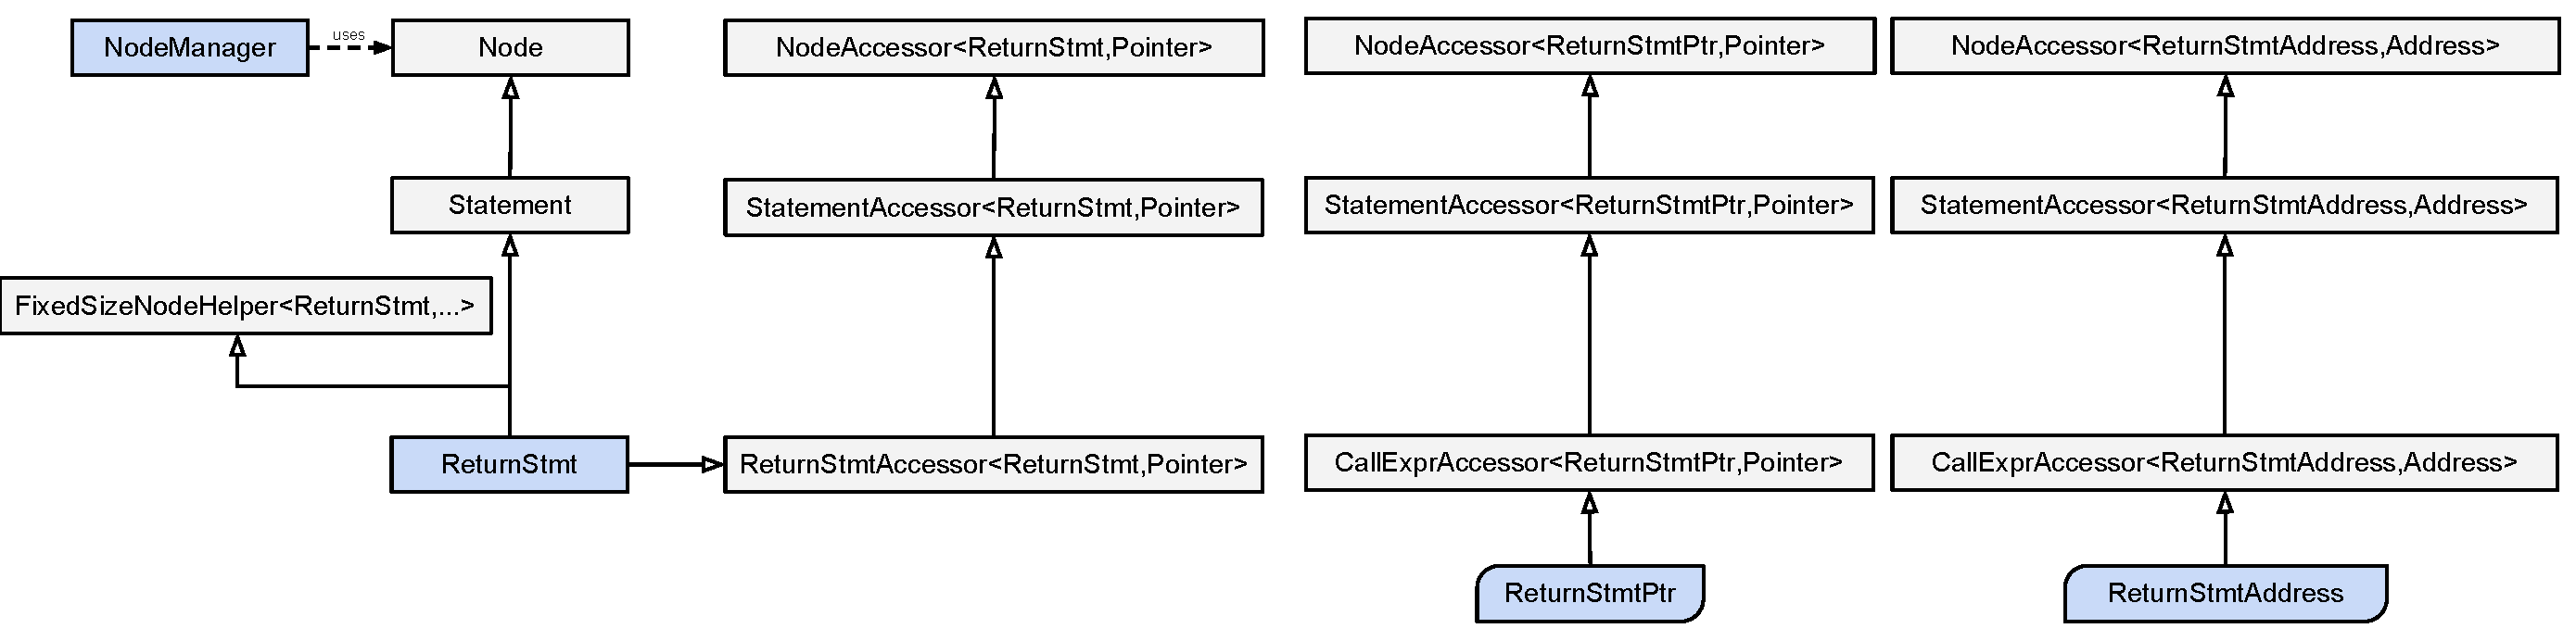
\includegraphics[width=\textwidth]{compiler/core/class_hierarchy_of_return_stmt.pdf}
	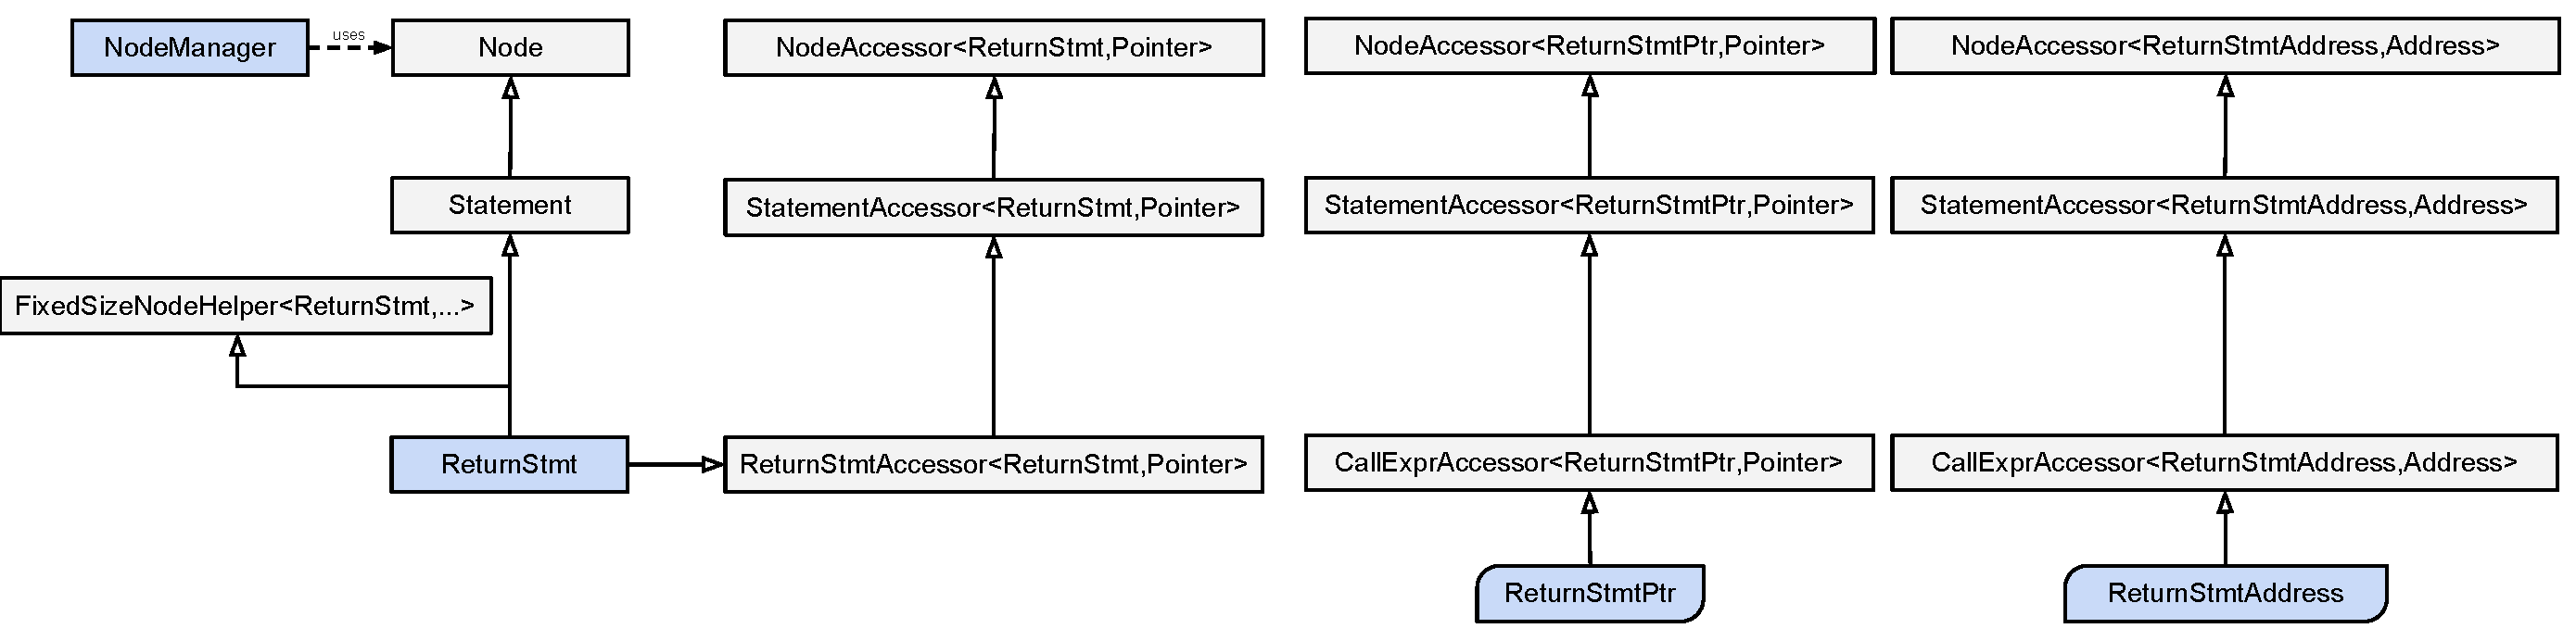
\includegraphics[width=\textwidth/4*3, trim=0 50 670 0, clip]{compiler/core/class_hierarchy_of_return_stmt.pdf}
	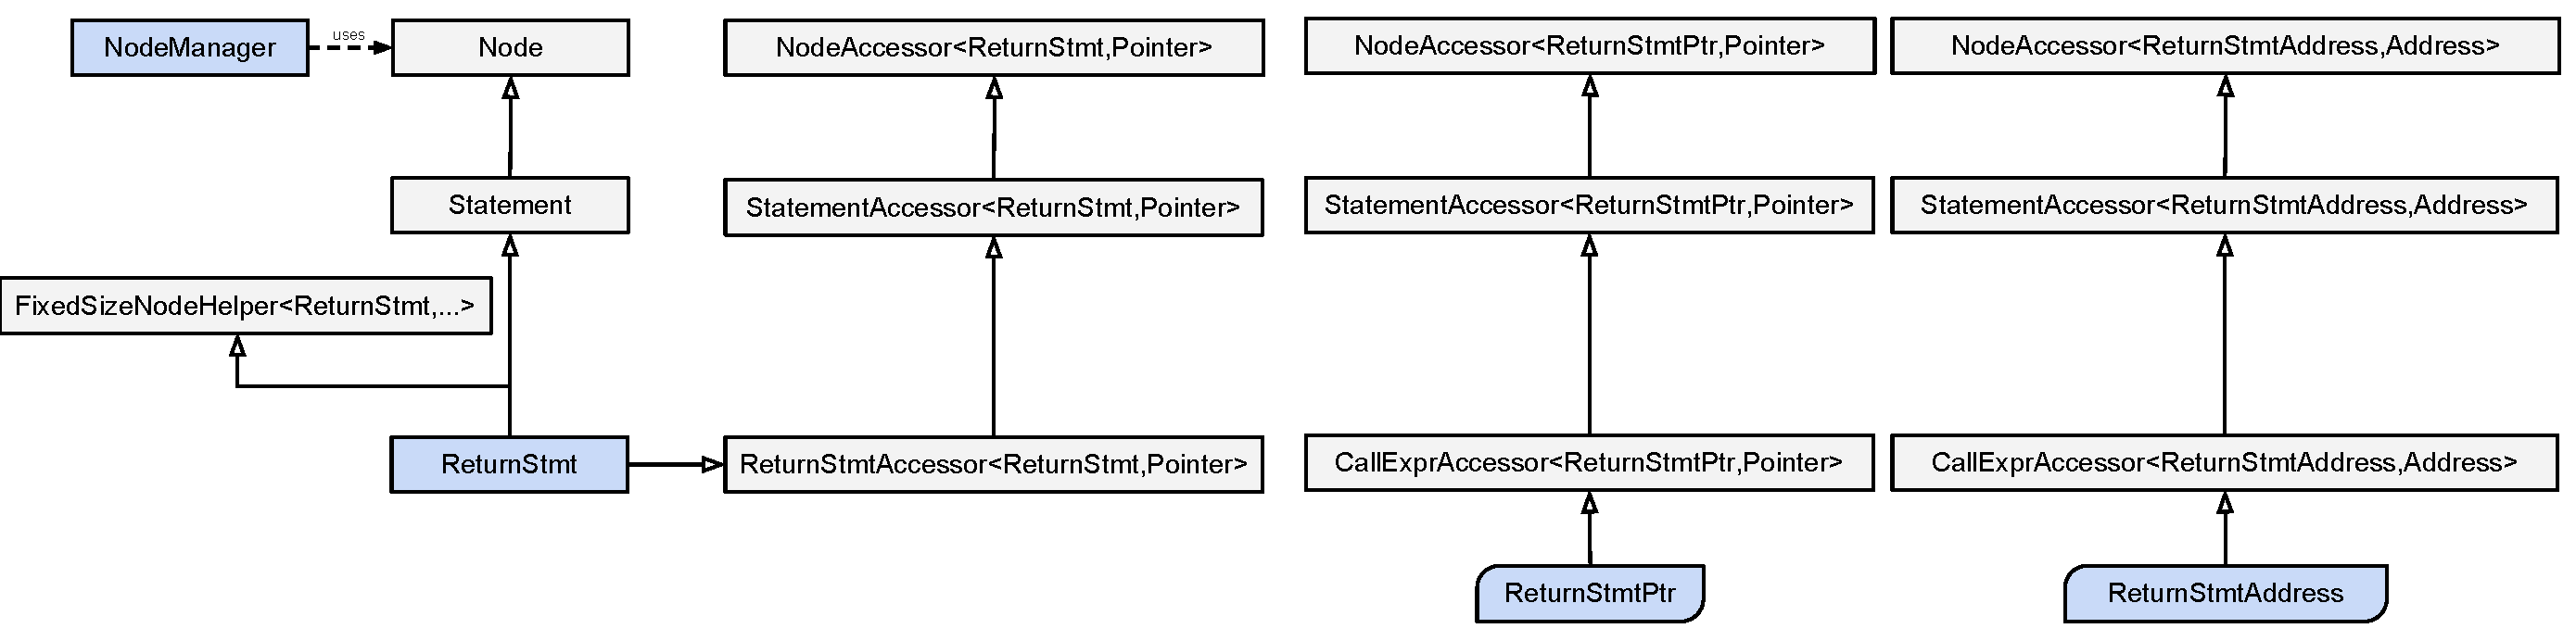
\includegraphics[width=\textwidth/4*3, trim=670 0 0 0, clip]{compiler/core/class_hierarchy_of_return_stmt.pdf}
	\caption{Relations between Classes contributing to the ReturnStmt}
	\label{fig:Compiler.Core.Classes.ReturnStmt}
\end{figure}
The blue boxes mark types being exposed to the user. The gray boxes are various
instantiations of generic types contributing the required functionality. The
following concrete classes are contributing to the architecture:
\begin{itemize}
  \item Node \ldots the generic base type
  \item Statement \ldots the common base type of all statements extending the
  node. This type inheritance allows Statements to be treated like any
  other Node.
  \item ReturnStmt \ldots the class implementing a return statement in the IR.
  IT is a extending the Statement type. It is only defining the type and a
  factory function (see code documentation), yet it does not define observer /
  getter methods.
  \item NodeAccessor \ldots a generic type defining all observer /
  getter methods applicable to nodes in general. The template is exploiting
  static dispatching for addressing requests to the actual instance derived from
  the generic base class. This way, overheads in memory requirements and
  execution time should be avoided. The second template parameter defines the
  reference type returned by involved getters. For more details on the
  parameters see the source code documentation \cite{insieme_source_doc}.
  \item StatementAccessor \ldots a generic accessor extending the basic
  NodeAccessor by all observer functions offered by any statement
  \item ReturnStmtAccessor \ldots a generic accessor extending the
  statement accessor by the extra functions offered by ReturnStmt nodes.
  \item ReturnStmtPtr \ldots the type of pointer used to reference ReturnStmt
  nodes. It uses the same hierarchy of generic types to obtain the required
  functionality as the node implementation itself does. However, it used
  different types to instantiate the offered generic parameters. Hence, every
  observer function only needs to be implemented once -- in a generic context.
  \item ReturnStmtAddress \ldots the address based counterpart of the
  ReturnStmtPtr
  \item FixedSizeNodeHelper \ldots a generic variadic template utility class
  implementing type save accesses to members of the child list -- which forms
  the foundation for all observer functions defined within the Accessors.
\end{itemize}


In the implementation two types of nodes are distinguished. The first, the
\textit{FixedSizeNode} \index{IR!FixedSizeNode} type covers nodes having a fixed
size list of arbitrarily typed child nodes (like a tupel). For instance, the
ReturnStmt is a FixedSizeNode having a single child node -- the expression
computing the value to be returned. The second type is the \textit{ListNode}
\index{IR!ListNode}.
In addition to a fixed set of child nodes, ListNodes may have a variable length list
of child nodes of a homogeneous type. An example is the \textit{CallExpr}. It
child list has the shape
$$TypePtr, ExpressionPtr, ExpressionPtr^*$$
where the type is the type of the value represented by the call expression, the
first expression corresponds to the function to be called and the remaining
expressions to the arguments to be passed to the function. For ListNodes the
\lstinline|FixedSizeNodeHelper| is replaced by the \lstinline|ListNodeHelper|
and an additional layer of a \lstinline|ListNodeAccessor<>| class is introduced
at the bottom of the accessor hierarchy to support type-safe accesses to the
tailing node list. Figure \ref{fig:Compiler.Core.Classes.CallExpr} illustrates
the resulting class hierarchy of the CallExpr.
\begin{figure}[!tb]
	\centering
	%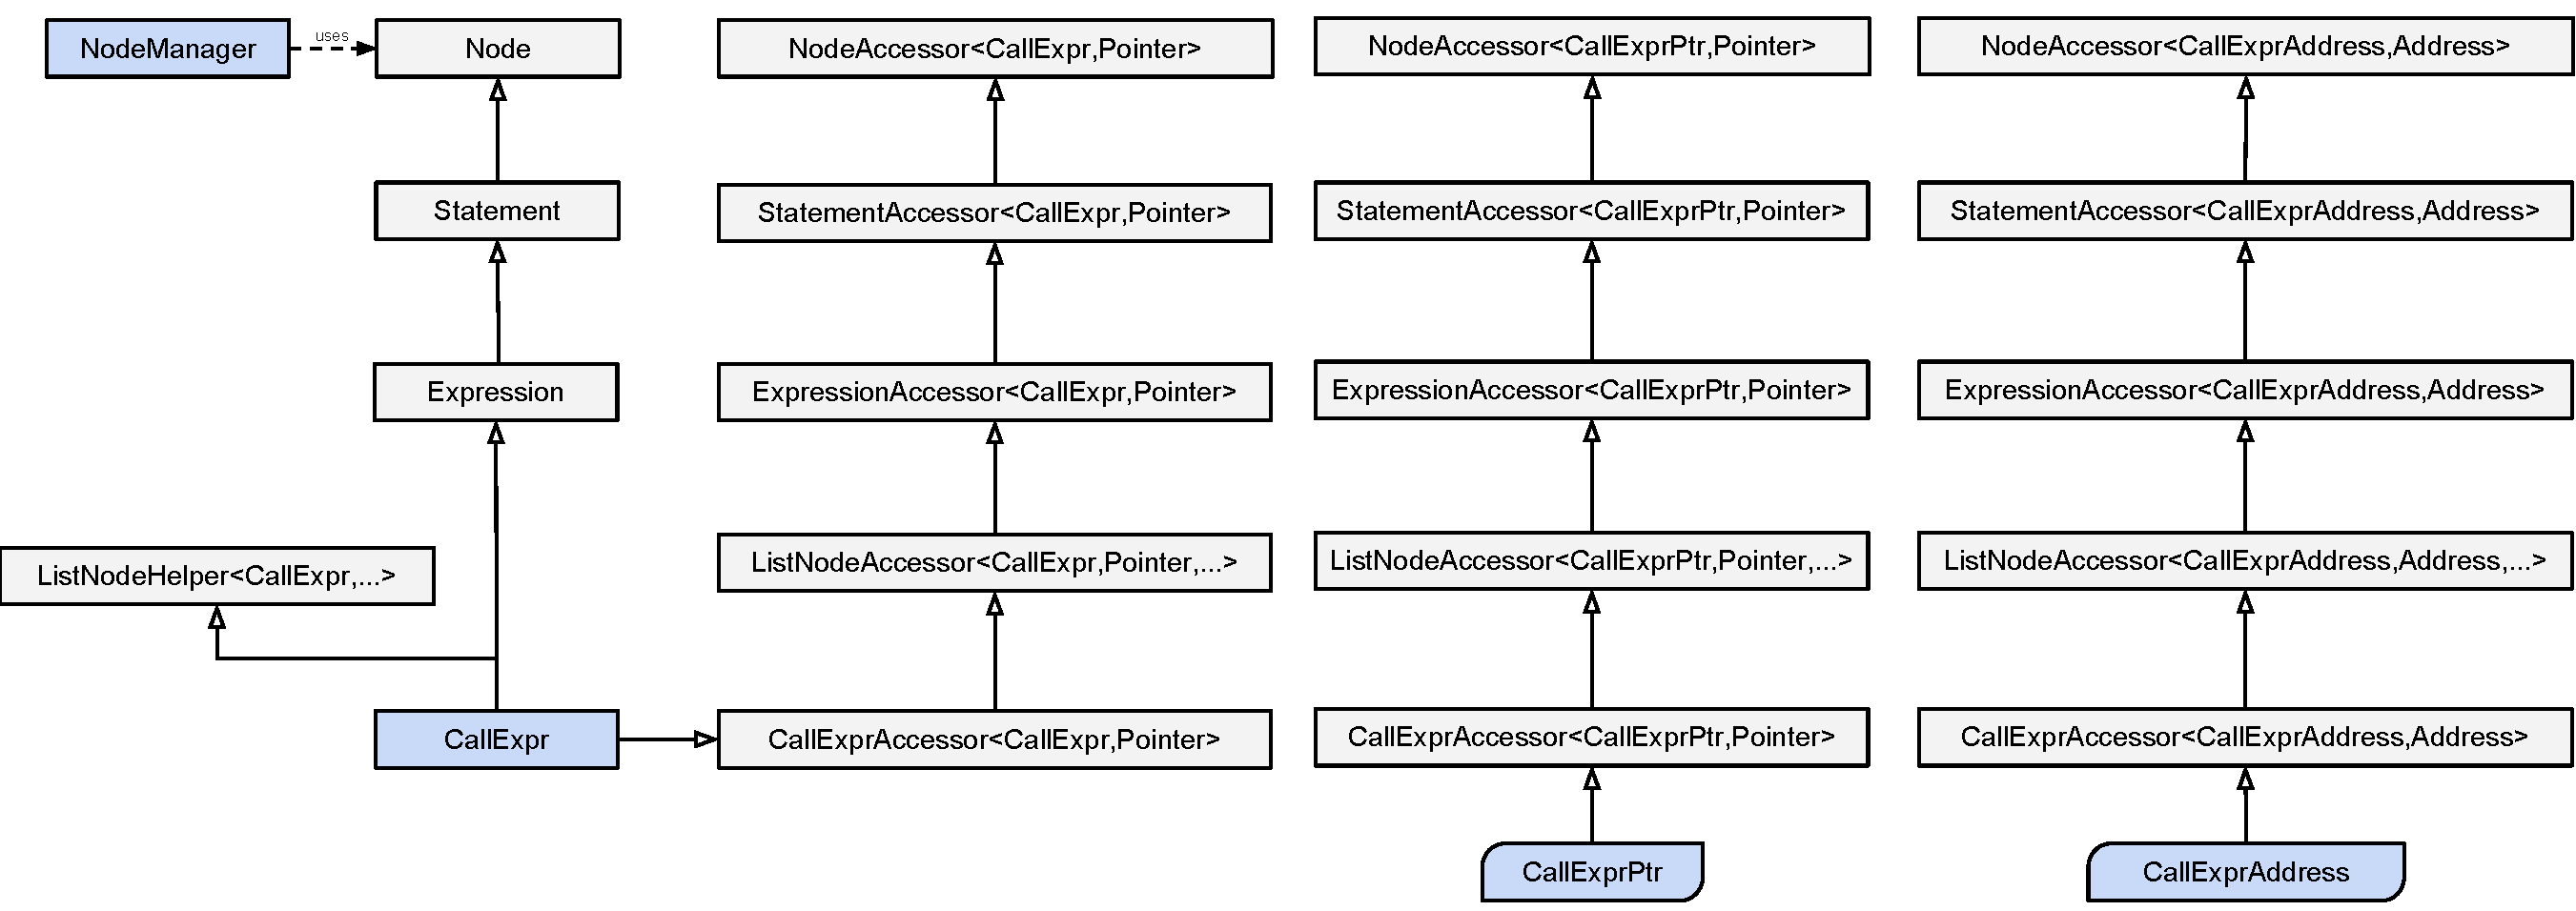
\includegraphics[width=\textwidth]{compiler/core/class_hierarchy_of_call_expr.pdf}
	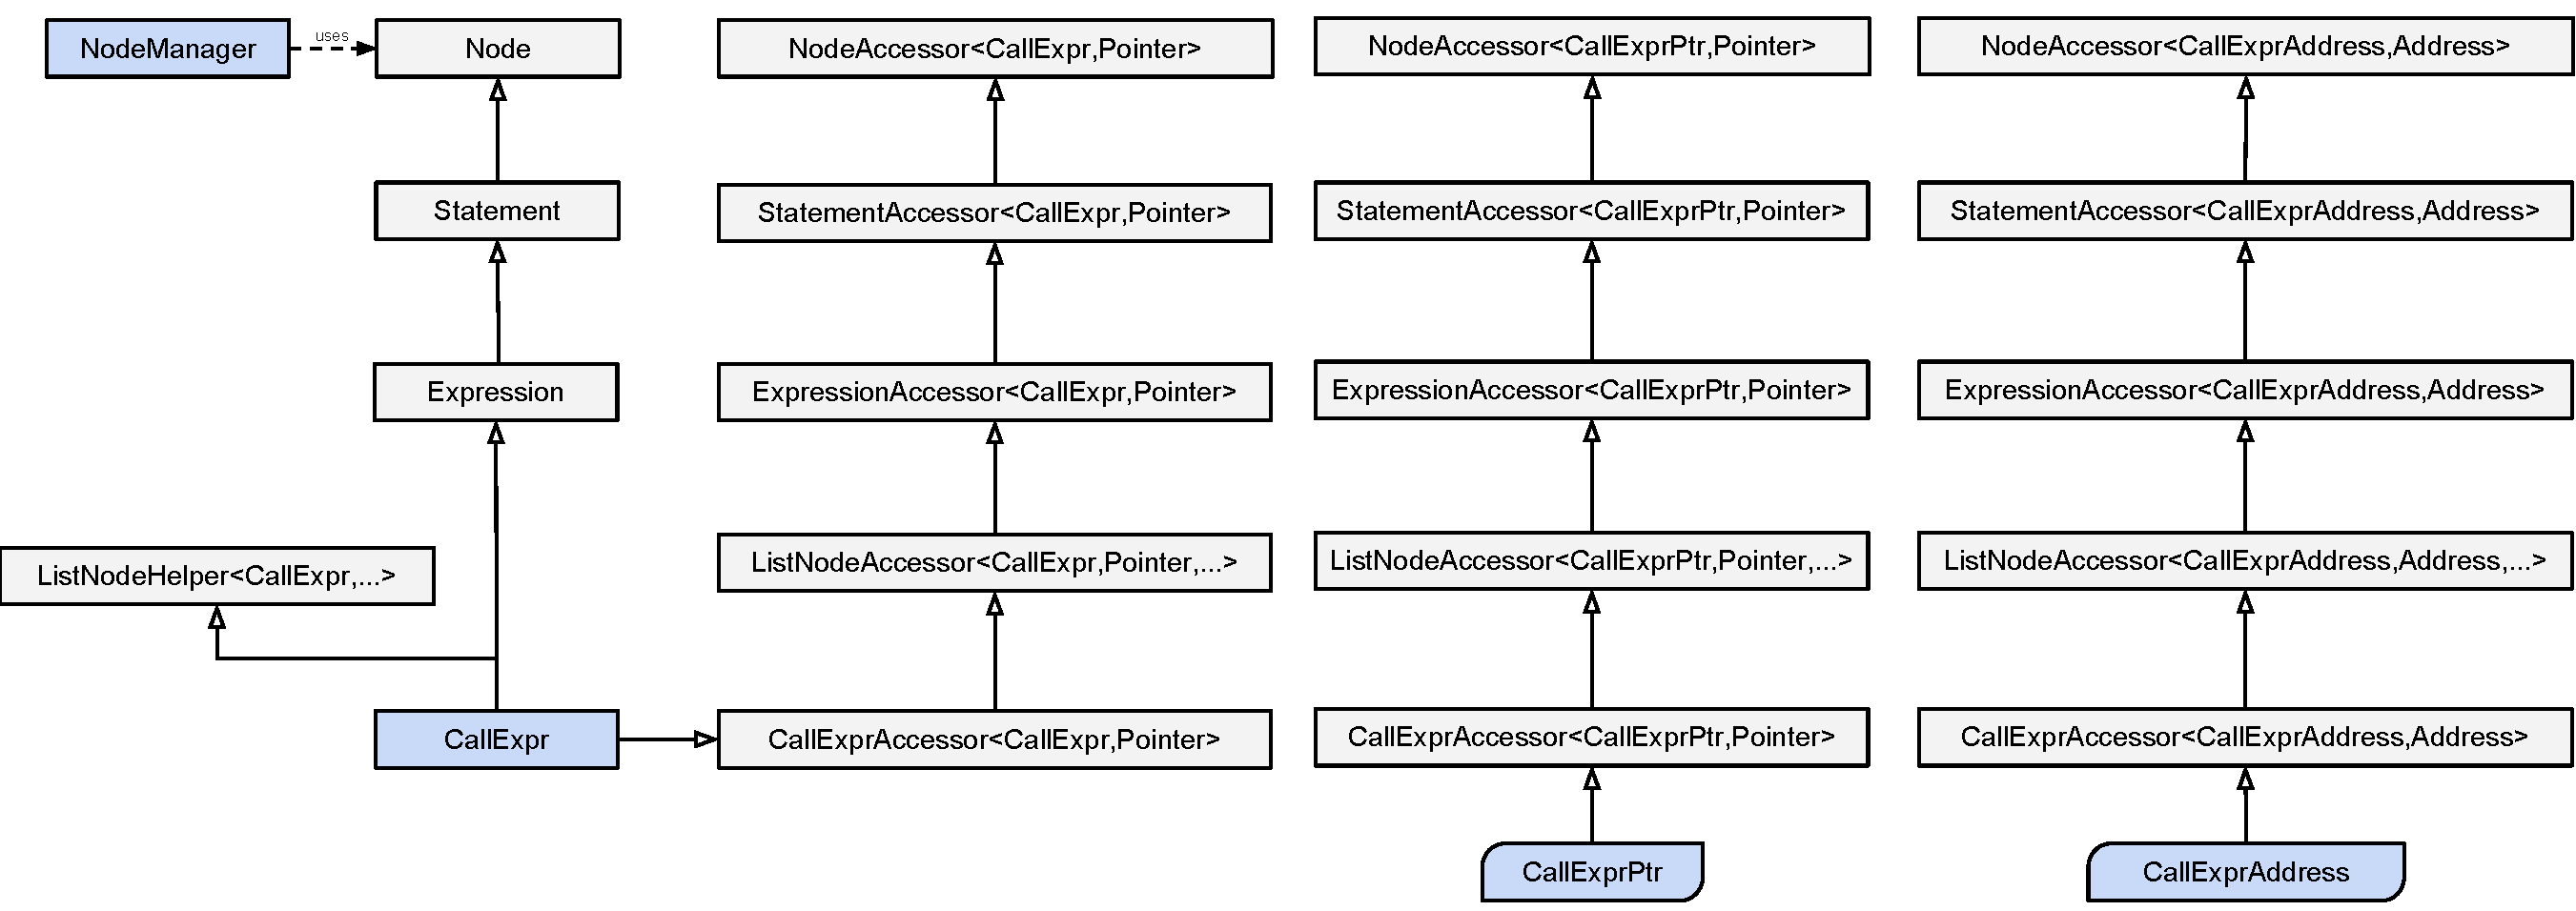
\includegraphics[width=\textwidth/4*3, trim=0 50 650 0, clip]{compiler/core/class_hierarchy_of_call_expr.pdf}
	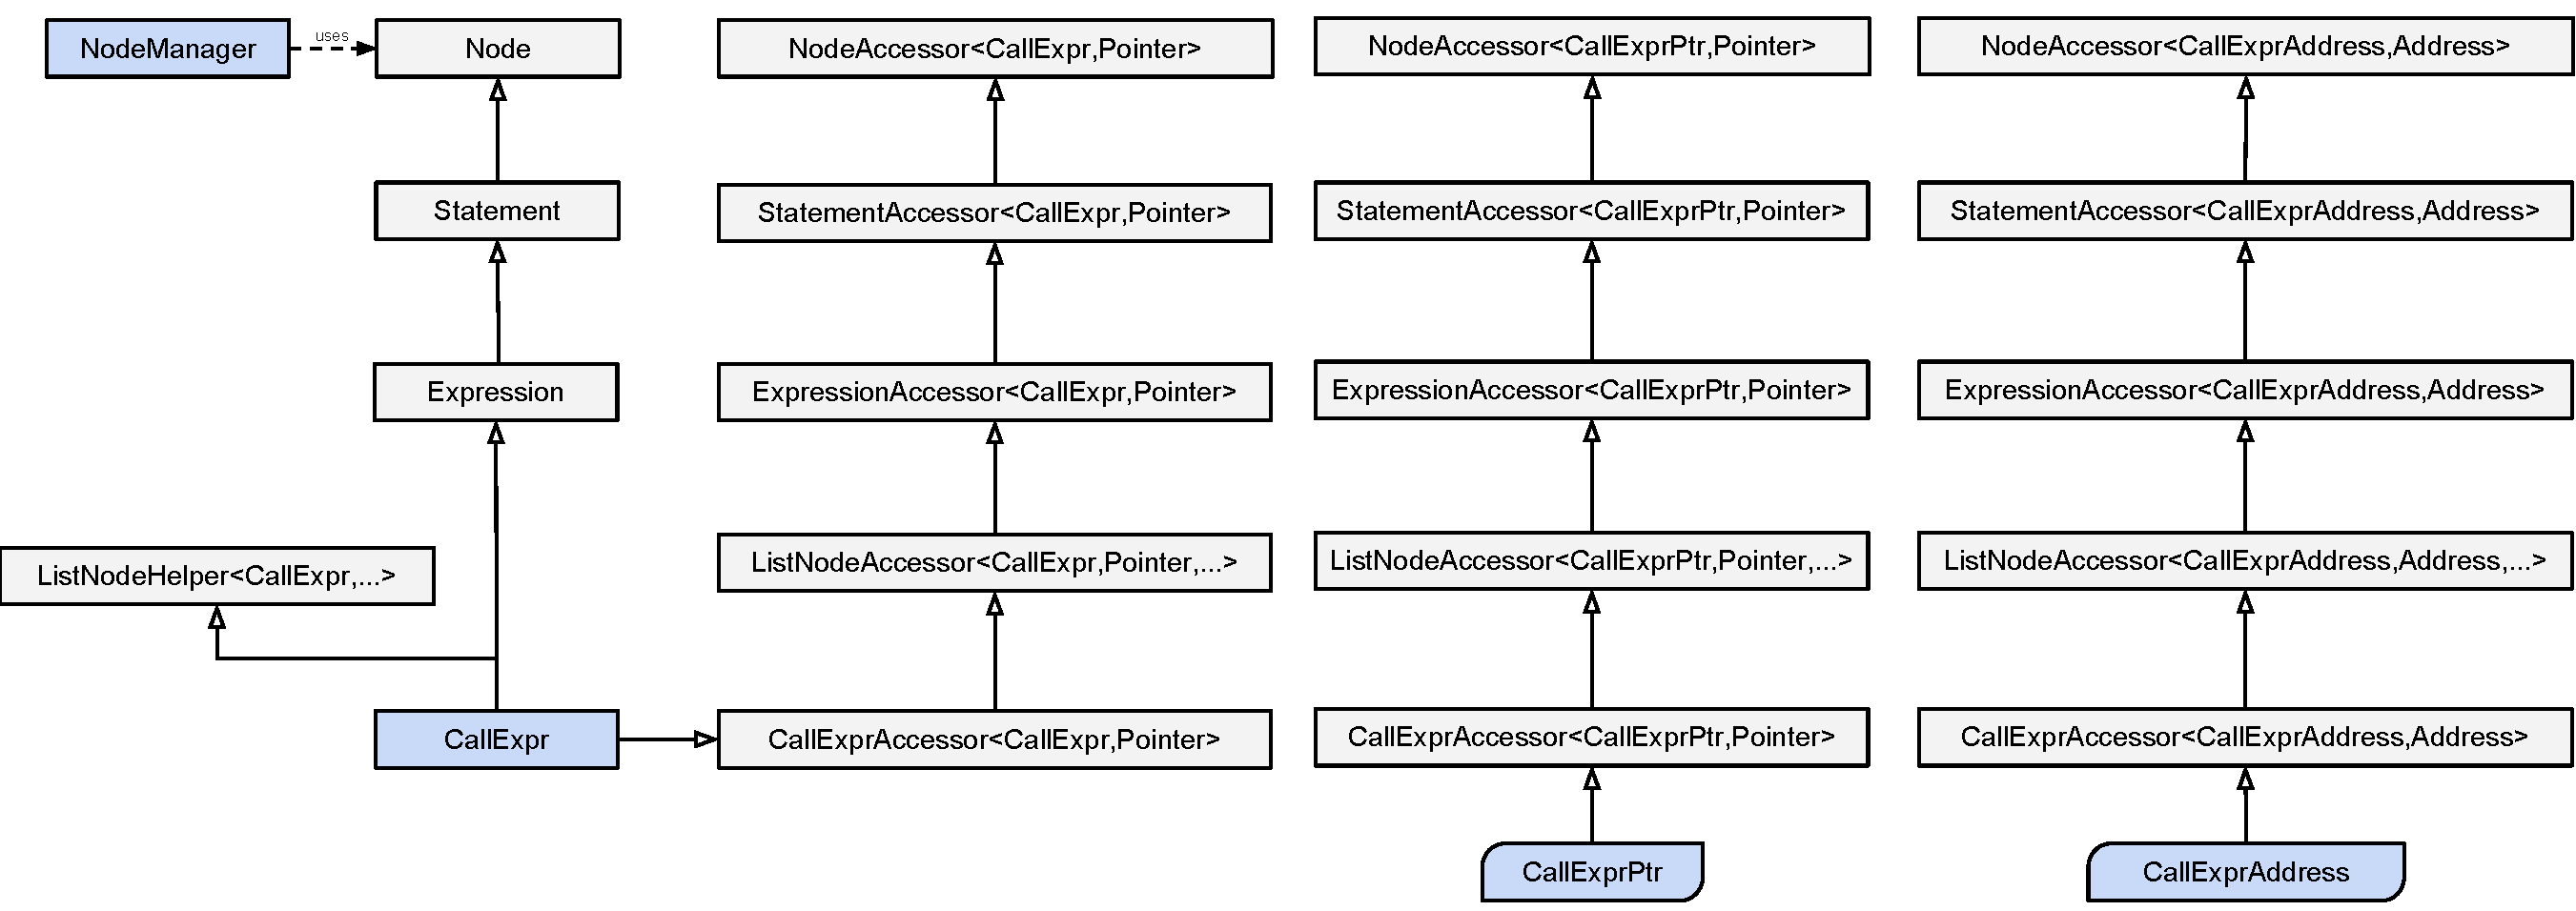
\includegraphics[width=\textwidth/4*3, trim=650 0 0 0, clip]{compiler/core/class_hierarchy_of_call_expr.pdf}
	\caption{Relations between Classes contributing to the CallExpr}
	\label{fig:Compiler.Core.Classes.CallExpr}
\end{figure}
Note: although the CallExprPtr type inherits from 5 classes it is not virtual.
It also just requires the size of a single pointer in memory and does not
introduce any overhead for construction / destruction except of setting the
pointer-member field. This light-weight property is especially desirable
when considering the fact that instances of NodePointers are created and
destroyed billions of times when running compiler code.

\subsubsection{Macros}
The restrictions imposed on nodes makes the implementation of the actual
instances a quite mechanical task -- and is therefore left to marcos. Within
\textit{ir\_node.h} the following Macros are defined to generate node Accessors
and Node Implementations: 
\begin{itemize}
  \item IR\_NODE \ldots creates the head of a Node
  type definition including classes to be extended and a set of required constructors and a default
  factory. This Macro should be used to define new Node classes and extend those
  by static factory methods. 
  \item IR\_NODE\_ACCESSOR \ldots creates
  the head of a NodeAccessor definition for a FixedSizeNode including all
  dependencies and some member type definitions. The macro accepts a variable
  length argument list which has to be instantiated by the list of types
  expected to form the child list of the corresponding node.
  \item IR\_LIST\_NODE\_ACCESSOR \ldots the same as the IR\_NODE\_ACCESSOR
  macro, yet generating a NodeAccessor definition header for ListNodes.
\end{itemize}
However, those might only be used for creating
concrete nodes (nodes forming leafs of the type hierarchy, e.g. CallExpr), not
for abstract nodes within the type hierarchy (e.g. Statement, Expression,
\ldots). Those need to be implemented manually. For an extensive set of examples
on their application readers are referred to the existing node implementations.

\subsubsection{The NodeType Enumeration}
The X-macro file \textit{ir\_nodes.def} defines the list of all existing node
types and their direct inheritance relation ship. It is used at various places
for statically generating codes depending on this information using the C
pre-processor. An example case is the definition of the NodeType enumeration
within \textit{ir\_node\_types.h}. 

Every node instance is exposing its type via the \lstinline|getNodeType()|
method (defined within the generic NodeAccessor). This function can therefore be
used to determine the type of a node.


\subsubsection{Special Algorithms}
Within this subsection a view specific algorithms involved in the managing of
nodes will be discussed. 

\paragraph{Implicit Node Sharing} \index{IR!Node Sharing}
The virtual IR trees are internally maintained as a DAG by sharing identical
sub-trees. To realize this, a mean allowing to determine whether a certain node
instance already exists. This is one of the roles of the NodeManagers (beside
the life-cycle management).

The InstanceManager, a generic utility class the NodeManager is based on, is
maintaining a set of all nodes currently ``alive'' within his domain. This set
is based on a hash. Therefore, every element within the set has to offer a hash
value and an equality function. Both requirements are realized by the Node base
class (which is possible do to the constraints defined by
\ref{eq:Compiler.Core.NodeDef}).

Whenever a Node is created, the following procedure is conducted:
\begin{enumerate}
  \item The Type and the Child-Node List is obtained (e.g. via an argument of
  the factory function)
  \item A local instance of the resulting node is created on the stack
  \item It is passed to the manager to obtain the ``master copy'' of
  requested node
  \item The manager computes the nodes hash value (by using one of its methods)
  to perform a look-up in its internally maintained set
  \item If present, the manager returns a reference to the obtained master copy
  \item If not present, a new master copy is created by cloning the handed in
  temporary node and a reference to the new node is returned
  \item The temporary copy on the stack is destroyed 
\end{enumerate}

In the concrete case of a ReturnStmt all those steps are conducted within one of
its factory functions using the following line of code:
\begin{lstlisting}
	return manager.get(ReturnStmt(expression));
\end{lstlisting}

In the end, although the mechanism beneath is complex, the interface to the user
is kept as simple as possible. The node-sharing happens automatically.

\paragraph{Hashing} \index{IR!Hashing}
The hashing of Nodes is implemented within the static member function
\lstinline|hashNodes| of the Node class and the \lstinline|hash| functions
within the \textit{ir\_node.cpp}. All of them are simply combining the hash
values of the child nodes with the NodeType using a boost utility function to
obtain a proper hash code. Therefore, the hash value of a node recursively
covers the entire virtual sub-tree rooted by the given node.

Since hashes are depending on the entire sub-tree, computing those can become
expensive. In fact, the recursive computation grows exponential with the height
of the IR tree. Fortunately, all nodes are immutable. Therefore, hashes can be
cached and computed once during construction -- by only accessing the already
cached hash codes of the child nodes. This way, the computation of the hash is
reduced to a local operation, hence $\mathcal{O}(1)$;

\paragraph{Equality} \index{IR!Equality Classes} 
For the look-up in the HashSet Nodes need to be tested for equality. If two
nodes are equivalent, this is quite easy. With a probability bordering on
certainty their hash values will be different. If not, node types or the
immediate child nodes are likely to be different. Hence, inequality can be
quickly (almost always locally) decided.

However, in case two nodes (and hence the represented sub-trees) are equivalent,
this cannot be decided as effectively with the provided means. Just because hash
values are identical does not allow to conclude that the corresponding trees are
equal. To make sure two trees are identical, every node within one tree has to
be compared to every node within the other tree. Hence, deciding whether two
trees are equivalent is an expensive operation -- considering the fact that
trees may consist of more than 10 million (virtual) nodes for moderate sized
codes.

To fix this problem, equivalence classes of nodes identified by simple integer
IDs are formed dynamically to cache comparison results. The mechanism is
implemented by the == operator of the Node class. Each node is created using an
equality class ID of 0 (hence, no class fixed yet). If it is ever compared to
another node and determined to be equivalent, the equality ID of the other node
is copied. If the other ID is also 0, a fresh equality ID is assigned to both
nodes. Future comparisons start by comparing the equality ID.
If both are not 0 and equal it can be immediately deduced that nodes are equal. If both are
not 0 and distinct, the comparison has to be continued recursively (they still
might be equal, just their equality classes never ``met'' so far). Finally, in
case two nodes are determined to be equivalent although their equality ID is set
and distinct, the larger equality ID will be replaced by the smaller one. This
way, equality classes are merging over time.

The locally stored integer allows to determine equality effectively using
locally available information. Even in the cases the local nodes does not have a
set equality ID, it is likely the child nodes have. Amortised, this should
result in a complexity of $\mathcal{O}(1)$ for determining whether two IR trees
are structurally identical.


  

\subsubsection{HowTo}
Finally, to conclude the documentation of the Node implementation some example
of common steps should be documented:

 \paragraph{Add a new Node} When ever adding a step, follow the following
 procedure:
 
\begin{enumerate}
  \item Do you really need a new node type or would a type, function or
  combination of existing nodes be sufficient?
  
  \item So, you're serious, you really need a new one? If not, just stop here.
  
  \item Register the new Node within the type hierarchy within
  \textit{ir\_nodes.def}. This will automatically create an entry in the
  NodeType enumeration, add support within visitors, IR statistics and printers.
  
  \item Determine whether your new node is a FixedSizeNode or a ListNode.
  
  \item Pick a file to implement your new node. In the header file you have to
  define the accessor and the node class itself. Use the corresponding macros
  defined within \textit{ir\_node.h}. When defining the accessor, fix the list
  of child node types.
  
  \item Add a list of accessor functions to the accessor using the
  IR\_NODE\_PROPERTY macro. Each macro is mapping a type and name to a certain
  location within the child-node list.

  \item If necessary you can add derived accessors (accessing nodes of
  child-nodes). For examples see the implementation of the ForStmtAccessor.
  
  \item Add required factory functions to the body of the node class definition.
  
  \item Rerun the cmake-script to trigger the IR builder generator (see
  \ref{sec:Compiler.Core.Builder} for details)
  
  \item Test your new node. You may extend one of the existing test cases.
  Essentially, would should be at least (!) done is to create an instance -- or
  more if complex combination of child lists are possible -- and run the
  \lstinline|basicNodeTests| implemented within \textit{ir\_node\_test.inc}
  located in the test folder of the core project.
\end{enumerate}
 
 
\paragraph{Add a Member Field to a Node Type}
To add a new property to a node, process the following steps:
\begin{enumerate}
  \item Determine whether the new field requires a new entry in the child-list
  or whether it is a derived one.
  
  \item If derived: use the examples included within the ForStmt
  (for deriving nodes) or the LambdaExpr (for derived non-node
  values) implementations as an example
  
  \item If a new filed:
	\begin{itemize}
	  \item add the type of the new field to the child-type list
  	  within the corresponding NodeAccessor
  	  
  	  \item add a access method using the IR\_NODE\_PROPERTY macro

  	  \item if the new child node has not been appended to the end, fix the
  	  indexes of the remaining methods

  	  \item update the factory function, which will update the builder when
  	  running cmake the next time

  	  \item fix all depending utilities like the pretty printer, the backend or
  	  any code using the factory function (if not backward compatible)
	\end{itemize}
  
  \item Extend the existing test cases to cover the new node
\end{enumerate}

\paragraph{Add a Method to a Node Type} 
To add new method to a node, you should first think whether your desired
operation is of general interest -- hence, whether it has a wide enough
relevance to justify adding it to the node itself instead of realizing it
as a function within some external utility header. The node implementation
should be kept clean of use-case specific codes.

If you decide that your method is important / useful / convenient enough, you
should add it using the same procedure as has been described for derived members
within the previous HowTo. As an example you can have a look at the
\lstinline|isRecursive()| method of the \lstinline|LambdaExpr| node.


\paragraph{Migrate Codes between Node Managers}
When working with multiple node managers frequently the question regarding how
to migrate an IR DAG from one node manager to another. The answer is simple:
just ask the target manager for a reference to the corresponding IR structure.

For instance, let \lstinline|code| be a reference (NodePtr) to the root of some
IR structure. Let \lstinline|targetMgr| be the manager you want to obtain a copy
from it. Simply use 
\begin{lstlisting}
	auto copy = targetMgr.get(code);
\end{lstlisting}
to obtain the corresponding copy within the target manager. If your
\lstinline|nodeAddr| is of type \lstinline|NodeAddress| (or any other node
address) you can use 
\begin{lstlisting}
	auto copy = nodeAddr.cloneTo(targetMgr);
\end{lstlisting}
to obtain a lone of the address within the given target manager. Unlike the
pointer variant, this does not only clone the addressed node to the target
manager but also all the nodes along the path described by the address,
in particular including the root node.

\paragraph{Use multiple Node Managers in Parallel Contexts}
Although generally immutable, the managing of nodes within the manager and the
handling of annotations is not synchronized. \note{This is something which
really should be fixed in the future!} Therefore, when operating on IRs in
parallel including the creation of nodes, each thread has to work on its own
copy using a local (private) node manager. 

Therefore, just create a local NodeManager and clone the IR to be processed to
your local manager. Further on you can run your operations in parallel on the
individual clones. Attention: if you want to return a value, you have to copy
the result back into the original NodeManager -- which should happen in a
synchronized way.

Some operations operating on IR nodes require the generation of fresh IDs (e.g.
variable IDs). Those IDs are managed by the NodeManager. After creating a local
manager, the next ID will be 1 again -- since none has been assigned yet.
Further, cloning IR structures into the manager will not change this
circumstance. In rare cases it can happen this way that presumably unique IDs
are used for new nodes which further on produce collisions since the same IDs
have been used before.\note{This is also something which should be fixed
soon. (I bet this note will be here forever)}

To prevent this from happening, after creating your private NodeManager the
fresh-value ID should be seeded. This can be conducted using the following code
snippet (also includes the parallel node manager creation):
\begin{lstlisting}

	core::StatementAddress trg = someSource(...);
	
	#pragma omp parallel
	{
		core::NodeManager local;
		core::StatementAddress localTargetCopy;

		#pragma omp critical
		{
			local.setNextFreshID(trg->getNodeManager().getFreshID());
			localTargetCopy = trg.cloneTo(local);
		}
	
		// run parallel operations

	}
	// temporaries automatically cleaned up
\end{lstlisting}


\begin{comment}
The main obligation of the core is to provide the data structures to model 

Sections:
\begin{itemize}
  \item General idea of the DAG and the sharing
  \item Involved classes and files and their relationship
  \item Implementation details of the classes
  \item The various node types
  \item Special Algorithms - hashing, equality
  \item HOW-TOs
\end{itemize}


To be covered:
\begin{itemize}
  \item Purpose of Nodes - distinction to the IR Spec
  \item Fact that nodes form a DAG
  \item Node Identity specified by type + children or value (little formally)
  \item Node Manager concept for memory management and sharing
  \item Handling the node manager in parallel environments
  \item Implementation of nodes (macros and generics)
  \item List of involved files (nodes.def, ir\_nodes.h, ir\_types.h)
  \item NodeType, NodeCategory, Nodes, Values, Types, Expressions, Statements,
  Support, Program, Accessors, \ldots + relations
  \item How to add new nodes
  \item How to add a method to a node
  \item How to add a field to a node (when to do so - e.g. not if it is
  something identity critical)
  \item Hashing and equality determination.
\end{itemize}

\subsubsection{Types}
\subsubsection{Statements}
\subsubsection{Expressions}
\subsubsection{Support}
\end{comment}



\subsection{Of Pointers and Addresses}
\label{sec:Compiler.Core.PointersAndAddresses}

\subsection{The IR Builder}
\label{sec:Compiler.Core.Builder}
\subsection{The Parser}
\label{sec:Compiler.Core.Parser}
\subsection{Visitors}
\label{sec:Compiler.Core.Visitors}
\subsection{Mappers}
\label{sec:Compiler.Core.Mappers}
\subsection{Lang-Basic and Extensions}
\label{sec:Compiler.Core.LangBasic}
\subsection{The Printer}
\label{sec:Compiler.Core.Printer}
\subsection{The Dumpers}
\label{sec:Compiler.Core.Dumpers}
\subsection{The Type Deduction}
\label{sec:Compiler.Core.TypeDeduction}
\subsection{The Semantic Checks}
\label{sec:Compiler.Core.SemanticChecks}
\subsection{Analysing Utilities}
\label{sec:Compiler.Core.Analysis}
\subsection{Node Statistics}
\label{sec:Compiler.Core.Statistics}
\subsection{Manipulation Utilities}
\label{sec:Compiler.Core.Manipulation}
\subsection{IR Data Encoding}
\label{sec:Compiler.Core.Encoding}
\subsection{Arithmetic Utilities}
\label{sec:Compiler.Core.Arithmetic}



\section{Annotations}

\section{Frontend}
\label{sec:Insieme.Frontend}

The frontend of the compiler is responsible of parsing an input program written
in a specific input language and to produce an IR program which semantically
equivalent to the input code. Because the IR is generic, many different input
programming languages can be represented by it. However a frontend must be
specific to an input language.

In the current development stage of the Insieme compiler only one frontend
exists for C-like languages based on the LLVM/Clang compiler~\cite{clang}. This
frontend supports C and C++, and above that it can deal with C language
extensions which are for example utilized for OpenCL and OpenMP. Because the
language extensions are always defined on top of a valid C/C++ code, the frontend
parse the input code in 2 major steps. In the first step, the sequential part of
the code is treated and converted into IR data structures. During this process,
information of eventual code extensions is collected and stored internally to
the frontend. In the second step, language extensions encountered in the input
code are applied to the generated IR and the final IR program is produced.  

\subsection{Overview of the Insieme Frontend}
\label{sec:Insieme.Frontend.Overview}

The frontend's job is to convert the AST generated by the LLVM/Clang compiler
into the corresponding IR DAG. Before this conversion can take place, the AST of
an input C/C++ code has to be generated. An overview of the conversion chain
implemented in Insieme is depicted in Figure~\ref{fig:Frontend.Architecture}.
The major difference between how any C compiler works and Insieme starts here.
While a generic C compiler parses, analyzes and compiles each translation unit
of the input program separately (often for performance reasons); Insieme needs
to have the knowledge of the entire input program before the conversion can be
started. For example, in order to be constructed, a \type{CallExpr} node of
the IR needs a reference to the corresponding \type{LambdaExpr} node which
contains the body of the invoked function.  Therefore the \texttt{CallExpr} node
cannot be created before the invoked function has been converted. Because a
function body in a C program often refers to a function definition in a
different translation unit, all the content of the translation units composing
the input program needs to be collected before the IR conversion process can
start.  This part will be discussed in more details in
Section~\ref{sec:Insieme.Frontend.TranslationUnits}.

\begin{figure}[tb]
	\centering
	%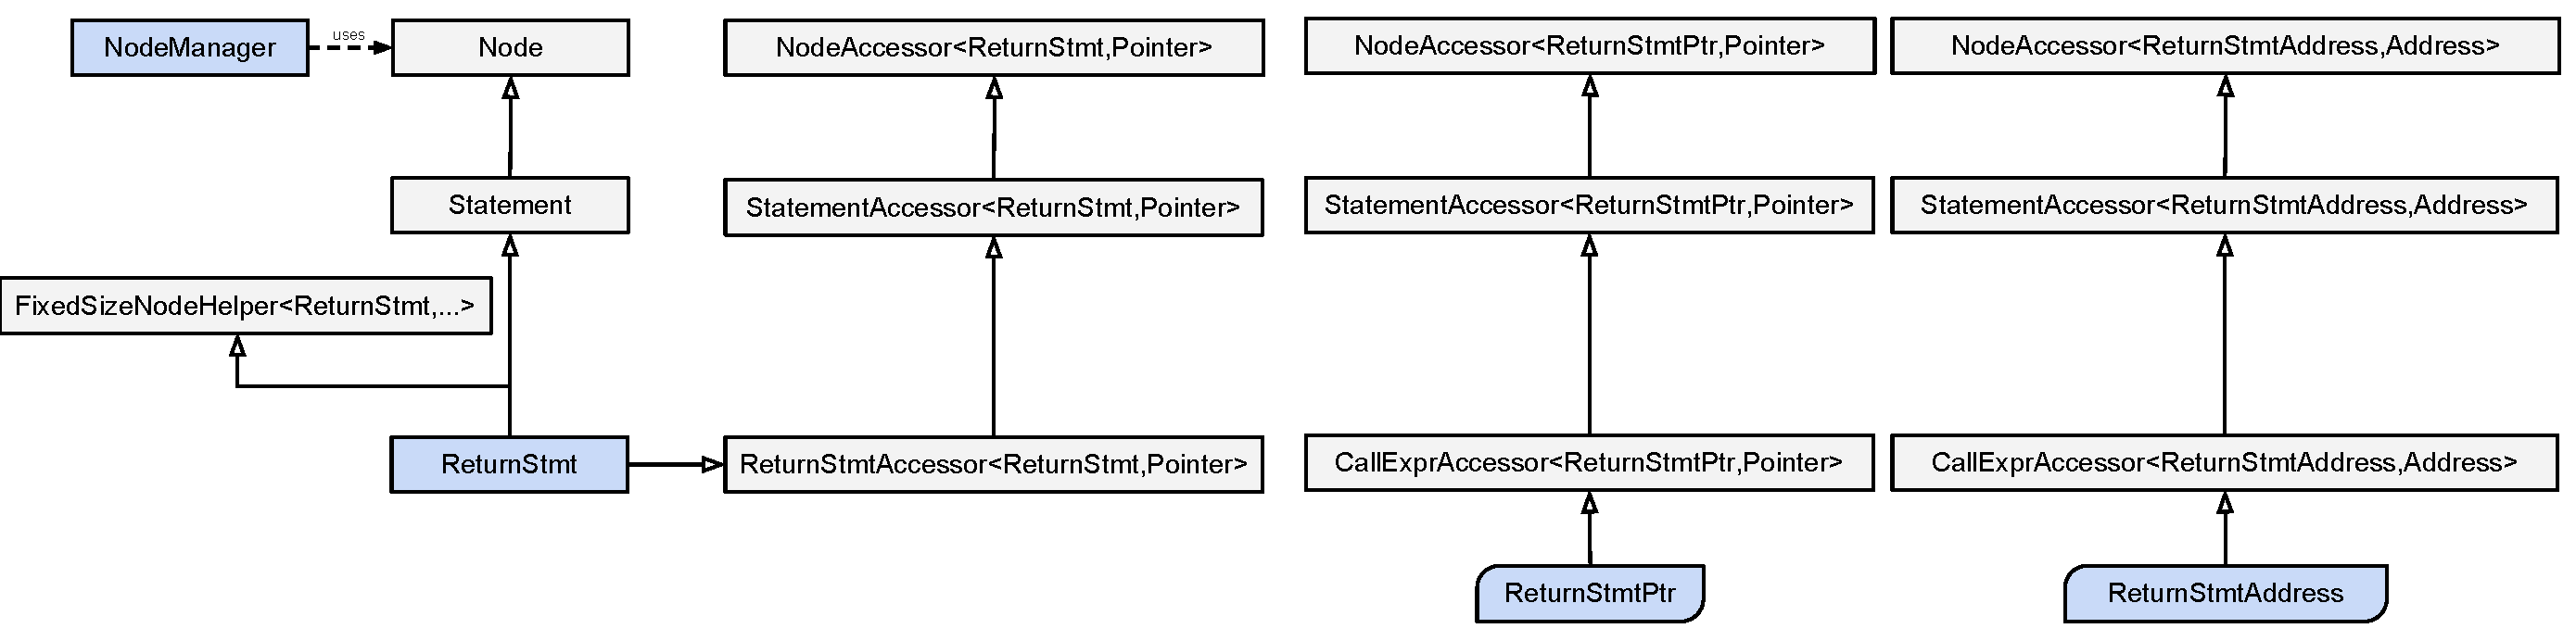
\includegraphics[width=\textwidth]{compiler/core/class_hierarchy_of_return_stmt.pdf}
	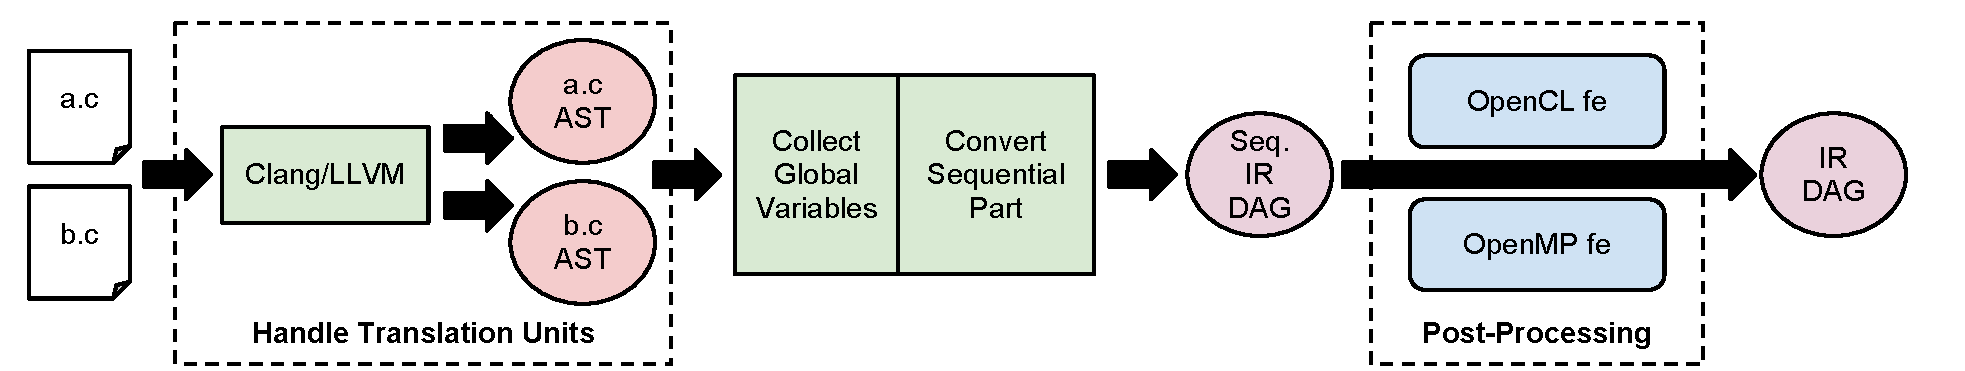
\includegraphics[width=\textwidth]{compiler/frontend/architecture.pdf}
	\caption{Overview of the frontend architecture}
	\label{fig:Frontend.Architecture}
\end{figure}

Once all translation units AST are in memory an analysis step on the entire
program is performed to capture eventual global and static variables in the
input code.  Indeed, because of the structural nature of the INSPIRE language,
variables are not referred by their name but instead by the DAG node
representing that variable. This makes it difficult to handle the semantics of
C/C++ \emph{global} and \emph{static} variables. In order to create a valid, and
semantically equivalent, IR program, the frontend needs to remove every global
variable from the program and accordingly replace them with plain variables
taking care of maintaining the semantics of the code. The details and
implementation issues related to the analysis phases performed for this issue
are discussed in Section~\ref{sec:Insieme.Frontend.Global}. 

Conversion of the Clang AST into an IR DAG is done using the well established
``Visitor'' design pattern~\cite{visitor-pattern}. The main idea is, for each
node of the Clang AST, to provide a transformation function which describe how
the C language entity (e.g. a variable declaration, an expression) should be
represented in the INSPIRE intermediate representation.  Management code makes
sure the generated IR nodes are automatically/correctly composed into a DAG. The
conversion of AST nodes of the C/C++ language is separated (for readability
issues) into 4 modules. 
\begin{description}
\item [\type{TypeConverter}] takes care of converting C/C++ data types (e.g. int,
array, struct) into the
corresponding IR types;
\item [\type{StmtConverter}] takes care of converting C statements (e.g. for, if,
switch) into the corresponding IR statements;
\item [\type{ExprConverter}] converts C expressions into IR expressions;
\item [\type{CxxConverter}] Converts C++ specific entities (e.g. virtual method
calls) into an IR representation.
\end{description}
These four modules are managed by the \type{ConversionManager} which is described
in Section~\ref{sec:Insieme.Convert}
While the conversion of most of the C AST nodes is straightforward and heavily
documented in the source code, one of the challenges in the frontend is the way
recursive types and functions are generated. Handling of such problem is treated
in Section~\ref{sec:Insieme.Recursion}.

One of the major features, and efforts, of the Insieme frontend is the handling
of user pragmas. Indeed, as part of the Insieme project, an engine for pragma
matching on top of the Clang compiler was developed. This framework allows for
user pragmas to be easily defined in EBNF form. The engine takes care of
matching those pragmas and store in a separate data structure, as node
annotations, the pragma information for later
consumption~\ref{sec:Insieme.Pragmas}. A use case is the implementation of the
entire OpenMP 3.0 standard on top of our framework~\ref{sec:Insieme.OpenMP}.

During the conversion the frontend stores in the IR nodes, using annotations,
several information which can be used by the middle- and back-end to gain more
knowledge of the input program. An example are OpenMP annotations which are used
to store the information contained in the OpenMP pragmas present in the input
code. In equivalent way, annotations are used to store OpenCL attributes whose
semantics is then handled in the OpenCL compiler~\ref{sec:Insieme.OpenCL}.

\subsection{Handling of Translation Units}
\label{sec:Insieme.Frontend.TranslationUnits}

INSPIRE represents input programs as a whole. This opposes to the way C programs
are usually written, by splitting the entire program into multiple files or
\emph{translation units}. In the trivial case when the entire program is
contained into a single source file, then the generation of the INSPIRE program
can be generated by examining that single file.

The Insieme frontend is shaped around the Clang compiler which provides the
utilities to perform syntactic and semantic analysis on the input code. Because
of performance reasons, the Clang compiler parses translation units separately.
An instance of the Clang compiler takes care of converting a C/C++ input file
into an AST which is internally represented by an object of the class
\type{clang::ASTContext} {\tt [\url{http://clang.llvm.org/doxygen/classclang_1_1ASTContext.html}]
} . In order to simplify the instantiation of Clang compiler instances, the
Insieme frontend implements a wrapper, {\tt ClangCompiler} defined in the
\file{frontend/compiler.h} header providing a simple way of retrieving a Clang
AST from an input file. The code which deals with the instantiation of a Clang
compiler instance and the setup of compilation flags being forwarded to Clang is
isolated in the \file{frontend/compiler.cpp} file. In the implementation code of
the \type{ClangCompiler} class we make sure that system include paths are
correctly set both for C and C++ headers. Several other flags are forwarded from
the Insieme input flags. 


\subsection{Handling of Global Variables}
\label{sec:Insieme.Frontend.Global}
\todo{week24}

\subsection{Conversion Manager}
\label{sec:Insieme.Convert}
\todo{week25}

\subsection{Recursive Type and Functions}
\label{sec:Insieme.Recursion}
\todo{week26}

\subsection{Matching of User Pragmas}
\label{sec:Insieme.Pragmas}
\todo{week27}

\subsection{OpenCL Frontend}
\label{sec:Insieme.OpenCL}

The OpenCL part of the Insieme frontend has two major responsibilities: On one hand it implements the semantics of many OpenCL library calls (in the OpenCL host code) and OpenCL built-in functions and implicit semantics (in the device code) to enable advantageous prgogram analysis. On the other hand, it connects the host and device code of an OpenCL program to form one single instance. Doing so, a lot of analysis and transformations can be done, which would not be possible when looking a both parts individually. One goal of the OpenCL frontend is to make all functinalities of the OpenCL library and built-in functions explicit, so that it an OpenCL program could be translated to a C program with the same semantics. \\

The transformations performed by the OpenCL frotnend are done entirely on INSPIRE level. This means, that the generic C/C++ frontend generates an IR DAG from the source code on which the OpenCL frontend performs some transformations, as shown in Figure~\ref{fig:Frontend.Architecture}. Qualifiers (e.g. \texttt{\_\_kernel}, \texttt{\_\_local}, \texttt{\_\_global}, etc.) which are not part of standard C are translated to \texttt{annotations::ocl::BaseAnnotation} with inside another annotation from the \texttt{annotations::ocl} namespace, depending on the qualifier (see Section~\ref{sec:Compiler.Core.Annotations} to read how and why annotations contain other annotations). The generic frontend is also responsible to translate OpenCL vector types to INSPIRE vectors with the appropriate type as well as translating vector accesses to subscript operations and operations on vectors (e.g. addition) to calls to the function \texttt{vector.pointwise}. This is done directly when translating the Clang AST to the INSPIRE DAG. \\

Since the OpenCL host code is just a standard C/C++ code which includes some specific headers whereas the device or kernel code uses an extension to a subset of C, the OpenCL frontend for both parts are implemented in two completely independend components which will be described in the following paragraphs. \\


\subsubsection{OpenCL Device Frontend}
\label{sec:Insieme.DeviceCL}

To be able to compile an OpenCL kernel function with Insieme, its file must include \texttt{ocl\_device.h}. This header file declares (but not implements) most of the OpenCL built-in functions, in both scalar and vector version. Since Clang version 3.0 the frontend shows some warnings about redeclaring some functions, since they are now built-in in Clang to. However Clang includes only very few functions, and of them it declares only one interface. Therefore this header file is still needed. When this header file is included in a kernel file, it cannot be compiled with an OpenCL compiler any more, since redefining all built-in funcitons leads to an error. Therefore it is a good practice to wrap the include inside \texttt{\#ifdef INSIEME} and to pass this definition to the call of the insieme compiler. 

Since the OpenCL kernels do not have a main function, the compiler is not able to find the entry points automatically. Therefore one must mark all kernel functions that should be compiled with Insieme using \texttt{\#pragma insieme mark}. The generic frontend will then generate a program with a separate entry point for each kernel functions and add an annotation which will be described in the next paragraph.

The transfromations necessary for the OpenCL device code are done in \texttt{ocl\_compiler.cpp}. The transformations are invoked by creating an object of type \texttt{insieme::ocl::Compiler} and invoking it's function \texttt{lookForOclAnnotations}. This functions walks through the program passed to its classe's constructor and searches for Nodes of type \texttt{NT\_MarkerExpr} which hold an \texttt{annotations::ocl::BaseAnnotation} with inside a \texttt{annotations::ocl::KernelFctAnnotationPtr}. This annotation is added by the C frontend to all functions which feature the OpenCL \texttt{\_\_kernel} qualifier. \\

When such a node is found the OpenCL host code transformations start on the child of the Marker Node. During these transformations the Marker Node itself will be removed while it's child will be replaced with a transformed version of it. The previously found \texttt{annotations::ocl::BaseAnnotation} will be attached to this newly generated node without any changes. \\

The most important task of the device frontend is to make the implicit parallelism of OpenCL explicit. When calling an OpenCL kernel, several instances of it will be started in a two level hirarchy of threads. The instances of the first level is called groups. Those gropus cosist of several work items (which are similar to threads). Both levels can have up to three dimensions. For a detailed description see~\cite{oclRef}. In order to capture this semantics in IR, two nested \texttt{parallel/job} constructs~\ref{parallel}[add ref to parallel constructs here] are wrapped around the kernel function's body, one covering the parallel groups, the other the parallel work items. Those \texttt{job} have a fixed range which is determined by the arguments \texttt{global\_work\_size} and \texttt{local\_work\_size} of the function \texttt{clEnqueueNDRangeKernel}. In OpenCL these values are passed to the kernel function impicitly, therefore in OpenCL we need to add two more arguments to the kernel to pass them explicitly. The number of theads of the outher parallel is equal to \texttt{global\_work\_size / local\_work\_size}. Therefore at the beginning of the kernel function, a statement performing exactly this calculation is added in order to use this as argument to the outher \texttt{job}. \\

The \texttt{parallel/job} constructs in INSPIRE are only one dimensional. Therefore the three dimensional thread grid of OpenCL simply flattend to generate two one dimensional spaces. In order to maintain the semantics of the input program, the three dimensional group/local or global id has to be restored at any place where an instance of \texttt{get\_[group|local|global]\_id} is called. In oder to do so, these functions are replaced with new functions, implemented in Inspire. Those new functions take not only the dimenson as argument (as their OpenCL counterparts do), but also the local/global size (passed as arguments to the kernel function as described in the prevous paragraph) and/or number of groups (calculated at the first line of the kernel, as described in the prevous paragraph), depending on the actual function. From these parameters the actual, 3D index is calculated using division and modulo calculations. Similarily, calls to \texttt{get\_[local|global]\_size} and \texttt{get\_num\_groups} are replaced with functions implemented in INSPIRE to give the same return value as the original ones.

Since adding \texttt{parallel/job} constructs introduces new scopes in INSPIRE, new variables have to be introduced in order to bring the values of the parameters of the kernel function to its body. The OpenCL Device Frontend does this 'bottom up' which means, that the ids of the variables inside the kernel body remain unchanged, while new variables are generated to be used in the parallel calls and as arguments. Furthermore, arguments which use the \texttt{\_\_local} or \texttt{\_\_constatnt} qualifier are added to the shared variable list of the jobs. Variables with a \texttt{\_\_global} qualifier are not added, since they are always pointer, and the pointer itself is private, only the data it is pointing to is shared among all treads. The declaration of local variables which use the \texttt{\_\_local} qualifier inside the kernel's body are moved between the two \texttt{parallel/job} constructs and the corresponding variables are added to the arguments of the inner \texttt{parallel} as well as to the shared variable list of the inner \texttt{job} to match the OpenCL semantics. 

When inside a kernel another function is called, the interface of this function may be changed. As mentioned before, in the INSPIRE represenation some functions need the local, global or group variable as argument which is not there in the OpenCL input code. Therefore, if anything inside a subfunction needs one of those variables, they will be added to the its interface and call.

In OpenCL all math functons (e.g. sin, cos etc.) can be marked as \texttt{native\_}. This keword means that, if awailable, a faster and less accurate version of the function (usually implemented in hardware) shall be used. To cover this semantic, the OpenCL Host Frontend removes the native from the function call and embeds it in a call to the function \texttt{accuracy.fast}, to keep the information that accuracy should be traded for speed if possible. This is also done for math functions marked as \texttt{half\_}. In OpenCL they use only two byte floating point numbers. But since Insieme does not support those and translates them to four byte floats, at least the fact that this function does not need high accuracy is preserved. The same is done for \texttt{mul24}. Since INSPIRE does not support \texttt{fma}, this function is expanded into a multiplication and an addition.

\texttt{mem\_fence} in OpenCL are directly translated into calls to \texttt{barrier} in INSPIRE. Mem fences on the local scope are mapped to barriers on the inner parallel while mem fences on global scope correspond to barriers on the outher (and therefore also inner) parallel region.

In OpenCL it is legal to assign a pointer of type \texttt{int} to another pointer of vector-type \texttt{int4} by using a simple cast. However this does not correspond with the semantics of a \texttt{CAST} in INSPIRE. Therefore, in such operations are replaced with a call to the function \texttt{ref.reinterpret}. This is already done in the generic frontend during the translation from Clang AST to the INSPIRE DAG. When one of the function starting with \texttt{convert\_} is used to transform scalar arrays to vectors, this function is not affected by the generic frontend but passed to the OpenCL Device Frontend. There it is replaced with a function which iterates over the array and constructs the desired vector element wise. Note: the function \texttt{ref.reinterpret} can not be applied here in general, since the soure may be not a reference.




\subsubsection{OpenCL Host Frontend}
\label{sec:Insieme.HostCL}



\subsection{OpenMP Frontend}
\label{sec:Insieme.OpenMP}





%\section{The Frontend}
%\subsection{The Frontend's Architecture}
%\subsection{The C Converter}
%\subsection{The Pragma Parser}
%\subsection{The OpenMP Frontend}
%\subsection{The OpenCL Frontend}
%\subsection{The MPI Frontend ?}
%\subsection{The C++ Frontend}
%\subsection{Customizing the Frontend}

\section{The Backend}
\subsection{The Backend's Architecture}
\subsection{The Sequential Backend}
\subsection{The Runtime Backend}
\subsection{The OpenCL Kernel Backend}
\subsection{The OpenCL Host Backend}
\subsection{Customizing the Backend}

\section{The Simple Backend}

\section{The Analysis Module}
\subsection{SCoP Analyses}
\subsection{Features}

\section{The Transformation Module}
\subsection{The Transformation Framework}
\subsection{Of Patterns and Generators}
\subsection{The Polyhedral Transformations}
\subsection{The Rule-based Transformations}

\section{The Machine Learning Module}

\section{The Driver}
\subsection{The Measurement and Instrumentation Utilities}
\subsubsection{Remote Execution}
\subsection{The Integration Test Loader}

\section{The XML Dump}
\section{The Playground}
